% Chapter Template

\chapter{OPC Unified Architecture} % Main chapter title

\label{Chapter3} % Change X to a consecutive number; for referencing this chapter elsewhere, use \ref{ChapterX}

%----------------------------------------------------------------------------------------
%	SECTION 1
%----------------------------------------------------------------------------------------

\section{Service Oriented Architecture}

Service Oriented Architecture is family of principles which recommends assembling of the composite application and any other systems from the independend parts servicing any kind of the service. 

Nowadays most of the information technologies are moving into web. With incomming Internet of Things into industry, this section is not an exception. 
Anyhow industrial applications may differ a lot from each other, there is tendency to connect them together to create a larger systems. Main connection between different systems is the SOA, principes which can connect technologies on a different platforms. This technology transfer alone control and regulation systems into the global solutions. 


On figure below is obvious how SOA converts monotlitic and not-scalable system into the much more clear solution. Creating of the same application using single atomic services leads into the system which is much more scalable, reconfigurable and independent modules servicing data supports also much more debugging abilities of service without need to shut down the whole system.

\begin{figure}[hbp]
\centering
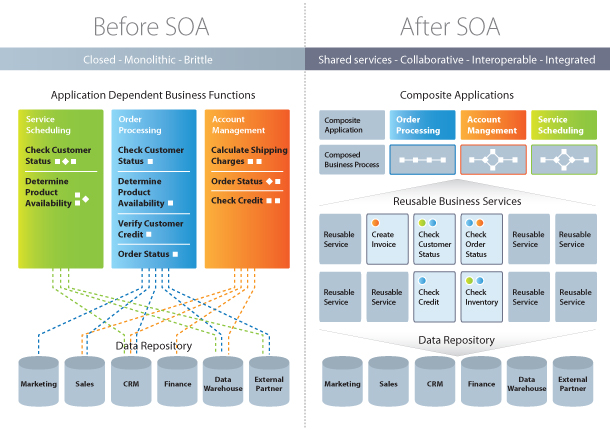
\includegraphics[scale=0.3]{Figures/diagram-soa}
\decoRule
\caption[4DIAC IDE Deployment Perspective ]{http://www.tridens.si/wp-content/uploads/2010/04/diagram-soa.jpg}
\label{4DIAC IDE Deployment Perspective}
\end{figure}


This approach brings re-usability feature, which is whole common in the other IT sectors, into the industrial systems.


\section{Web service}


Web service is a software system for communication of two computers in the network. It is described in a Web Services Description Language (WSDL). A Web service supports direct interactions with the other software agents using XML-based messages exchanged via Internet-based protocols. \cite{raey} Often the web port 80 is used to transfer data. This port is used mainly by web http protocol, so is opened on almoust every firewall. That is the huge advantage against any kind of proprietal ports. 


%-----------------------------------
%	SUBSECTION 1
%-----------------------------------
\section{OPC Unified Architecture}

Information system exceeds the borders of plant or event company, when companies are working together on common projects and products.
Due the huge demand of integration and interconnecting different control system the standardization is needed. Standardization of information systems reduces cost and time of integration. With standards comes also possibility to create generic adapters between any kind of systems. 

OPC Foundation answers this need of standardization. 
In the begining the OPC standed for OLE for Process Control. The OLE itself is Microsof proprietary technology called Object Linking and Embedding. This technology is used by Microsof to create references between the data objects in Windows OS. Microsoft later published SDK for this technology which leads to creation of the OPC. 

OPC Foundation decided to redesign OPC components and technologies with modern, vendor independent solutions.\cite{4618203}


The new specification is called OPC Unified Architecture (OPC UA). Nowadays the OPC means Openness, Productivity and Colaboration.


Currently, OPC is the communication standard in automation technology. Migration to OPC UA is needed to increase possible types of the integration solutions for which UPC can be used. This is achieved by using standard technologies to implement SOA and WS. 

\subsection{SOA in OPC UA}
OPC UA is based on SOA. OPC UA server contains set of services which are used by clients. These services provides all OPC UA functionality. 
Set of services available in any particular OPC UA server is defined in profiles that are described in OPC UA specification.

Each service call in IPC UA consist of a request and response message. 
In OPC UA there is a huge difference between services and methods. Wile services are strictly defined in the standard and user cannot change it, methods are user defined.
To invoke user-defined method on OPC UA server using service needed. 

\subsection{OPC UA communication stacks}
All the OPC UA standards are published by the OPC UA Foundation, but no official communication stack has been published yet.
OPC Foundation published just the example code in Java and Ansi C, but no complete SDK or even documentation.

However there are few open source or proprietary stacks available. 
On http://www.opcconnect.com/uakit.php#overview you can find Overview of Available SDKs and toolkits. 

There are also some open stacks for OPC UA. However these stacks are often published under license which is not compatible with 4DIAC license. 
I can mention OpenOpcUa which is open source, but to use it there is need to pay the one time fee. I can also mention FreeOpcUa hosted by the GitHub, but this sdk is not fully working and lack of documentation makes it almous impossible to use it for purpose of this thesis. However FreeOpcUa is C/C++ and Python SDK and in Python version much bigger progress is made. This SDK serves great open-source Python GUI interface for discovering the OPC UA server. 

Considering two important parameters license and documentation, open62541 stack seems to be optimal. This stack is used to integrate OPC UA into FORTE and will be described more in the below sections.

%-----------------------------------
%	SUBSECTION 2
%-----------------------------------

\section{OPEN 62541 stack}
Open 62541 is communication stack based on OPC UA standards published as IEC 62541 licensed under LGPL and free available on GitHub.

This stack is fully scalable, supports multi-threaded architecture, where every connection or session is operated by separate thread.

Open 62541 is written in C99 with POSIX support, so it is able to run on Windows, Linux, MacOS and Android. POSIX Linux support means open 62541 stack can also run on small embedded machines like raspberryPi, PLCs, etc.


\subsection{building sdk}
After downlaoding open 62541 stack sources from GitHub it is necessary to build them into header files. Also pre-generated sources and header files are available to downlaod. This pre-generated sources are just some demo with only basic functions like server, client and its basic functionality like read and write data. In this thesis also another functions like browsing across nodes on server and creating, editing and deleting nodes were needed, so in order to fullfil aim og this thesis specific sources were build. 

For detailed information about building library visit oficial documentation of open 62541.
http://open62541.org/doc/current/building.html



%----------------------------------------------------------------------------------------
%	SECTION 2
%----------------------------------------------------------------------------------------

